%%%%%%%%%%%%%%%%%%%%%%%%%%%%%%%%%%%%%%%%%
% Medium Length Graduate Curriculum Vitae
% LaTeX Template
% Version 1.1 (9/12/12)
%
% This template has been downloaded from:
  % http://www.LaTeXTemplates.com
%
% Original author:
  % Rensselaer Polytechnic Institute (http://www.rpi.edu/dept/arc/training/latex/resumes/)
%
% Important note:
  % This template requires the res.cls file to be in the same directory as the
% .tex file. The res.cls file provides the resume style used for structuring the
% document.
%
%%%%%%%%%%%%%%%%%%%%%%%%%%%%%%%%%%%%%%%%%

%----------------------------------------------------------------------------------------
  %  PACKAGES AND OTHER DOCUMENT CONFIGURATIONS
%----------------------------------------------------------------------------------------
  
  \documentclass[margin, 10pt]{res}\usepackage[]{graphicx}\usepackage[]{color}
% maxwidth is the original width if it is less than linewidth
% otherwise use linewidth (to make sure the graphics do not exceed the margin)
\makeatletter
\def\maxwidth{ %
  \ifdim\Gin@nat@width>\linewidth
    \linewidth
  \else
    \Gin@nat@width
  \fi
}
\makeatother

\definecolor{fgcolor}{rgb}{0.345, 0.345, 0.345}
\newcommand{\hlnum}[1]{\textcolor[rgb]{0.686,0.059,0.569}{#1}}%
\newcommand{\hlstr}[1]{\textcolor[rgb]{0.192,0.494,0.8}{#1}}%
\newcommand{\hlcom}[1]{\textcolor[rgb]{0.678,0.584,0.686}{\textit{#1}}}%
\newcommand{\hlopt}[1]{\textcolor[rgb]{0,0,0}{#1}}%
\newcommand{\hlstd}[1]{\textcolor[rgb]{0.345,0.345,0.345}{#1}}%
\newcommand{\hlkwa}[1]{\textcolor[rgb]{0.161,0.373,0.58}{\textbf{#1}}}%
\newcommand{\hlkwb}[1]{\textcolor[rgb]{0.69,0.353,0.396}{#1}}%
\newcommand{\hlkwc}[1]{\textcolor[rgb]{0.333,0.667,0.333}{#1}}%
\newcommand{\hlkwd}[1]{\textcolor[rgb]{0.737,0.353,0.396}{\textbf{#1}}}%
\let\hlipl\hlkwb

\usepackage{framed}
\makeatletter
\newenvironment{kframe}{%
 \def\at@end@of@kframe{}%
 \ifinner\ifhmode%
  \def\at@end@of@kframe{\end{minipage}}%
  \begin{minipage}{\columnwidth}%
 \fi\fi%
 \def\FrameCommand##1{\hskip\@totalleftmargin \hskip-\fboxsep
 \colorbox{shadecolor}{##1}\hskip-\fboxsep
     % There is no \\@totalrightmargin, so:
     \hskip-\linewidth \hskip-\@totalleftmargin \hskip\columnwidth}%
 \MakeFramed {\advance\hsize-\width
   \@totalleftmargin\z@ \linewidth\hsize
   \@setminipage}}%
 {\par\unskip\endMakeFramed%
 \at@end@of@kframe}
\makeatother

\definecolor{shadecolor}{rgb}{.97, .97, .97}
\definecolor{messagecolor}{rgb}{0, 0, 0}
\definecolor{warningcolor}{rgb}{1, 0, 1}
\definecolor{errorcolor}{rgb}{1, 0, 0}
\newenvironment{knitrout}{}{} % an empty environment to be redefined in TeX

\usepackage{alltt} % Use the res.cls style, the font size can be changed to 11pt or 12pt here
\usepackage{url}
\usepackage{hyperref}
\usepackage{helvet} % Default font is the helvetica postscript font
%\usepackage{newcent} % To change the default font to the new century schoolbook postscript font uncomment this line and comment the one above

\setlength{\textwidth}{5.1in} % Text width of the document
\IfFileExists{upquote.sty}{\usepackage{upquote}}{}
\begin{document}

%----------------------------------------------------------------------------------------
  %	NAME AND ADDRESS SECTION
%----------------------------------------------------------------------------------------
  
  
  
  %----------------------------------------------------------------------------------------
  
  \begin{resume}

\moveleft.5\hoffset\centerline{\Large\bf Karsten Tait Maurer}
\vspace{.15cm}
\moveleft.5\hoffset\centerline{\normalsize\bf Assistant Professor of Statistics}
\vspace{.1cm}
\moveleft.5\hoffset\centerline{\normalsize\bf College of Arts & Sciences Armstrong Interactive Media Studies Endowed Professor}
\vspace{.1cm}
\moveleft\hoffset\vbox{\hrule width\resumewidth height 1pt}
\vspace{.1cm}

%--------------------------------------------------------------------------
  % Full Contact Information %
  %--------------------------------------------------------------------------
  \section{CONTACT INFORMATION}

\begin{tabular}{p{5cm}p{5cm}}
Department of Statistics 
\newline Miami University 
\newline 321 Upham Hall 
\newline Oxford, OH 45056 

&

  \textit{Office:} 513-529-3404
\newline \textit{Email:} maurerkt@miamioh.edu
\newline \textit{Webpage:} \url{kmaurer.github.io}  \\

\end{tabular}

%----------------------------------------------------------------------------------------
  %	EDUCATION SECTION
%----------------------------------------------------------------------------------------
  
  \section{EDUCATION}

Ph.D., Statistics, 2015 \hfill Iowa State University, Ames IA  \\
M.S., Statistics, 2011 \hfill  Iowa State University, Ames IA  \\ 
B.A., Statistics and History, 2009 \hfill  University of Minnesota Morris, Morris MN 

%----------------------------------------------------------------------------------------
  %	Honors and awards
%----------------------------------------------------------------------------------------
%   \section{HONORS} 
% CAS Armstrong Interactive Media Studies Endowed Professor \hfill Summer 2018 \\

%----------------------------------------------------------------------------------------
  %  Sponsored Research Section
%---------------------------------------------------------------------------------------- 
  
  \section{SPONSORED RESEARCH}

ASA-NCTM Joint Committee [\$11750] - K12 Educators Workshop \hfill Summer 2019 \\
Air Force Research Lab [\$10000] - Research Extension Grant \hfill Fall 2018\\
Air Force Research Lab [\$15500] - Visiting Faculty Researcher \hfill Summer 2018 \\
Miami University [\$5000] - CAS Summer Research Appointment  \hfill Forgone 2018 \\
Miami University [\$5000] - CFR Summer Research Appointment  \hfill Summer 2017 \\
Air Force Research Lab [\$21500] - Summer Faculty Fellowship  \hfill Summer 2016 

%----------------------------------------------------------------------------------------
  %	PROFESSIONAL EXPERIENCE SECTION
%----------------------------------------------------------------------------------------
  
  \section{TEACHING}

Miami University, Oxford OH \hfill  Spring 2016-Fall 2018
\begin{itemize} \itemsep -2pt % Reduce space between items
\item STA 301, Applied Statistics (1 Section)
\item STA/IMS/JRN 404/504, Advanced Data Visualization (9 Sections)
\item STA 467/567, Statistical Learning (2 Section)
\item STA 477/600, Independent Studies in Statistics (7 students)
\item STA 671, Environmental Statistics  (1 Section)
\end{itemize}

\begin{center}
\begin{figure}[h!]
\hspace{-2cm}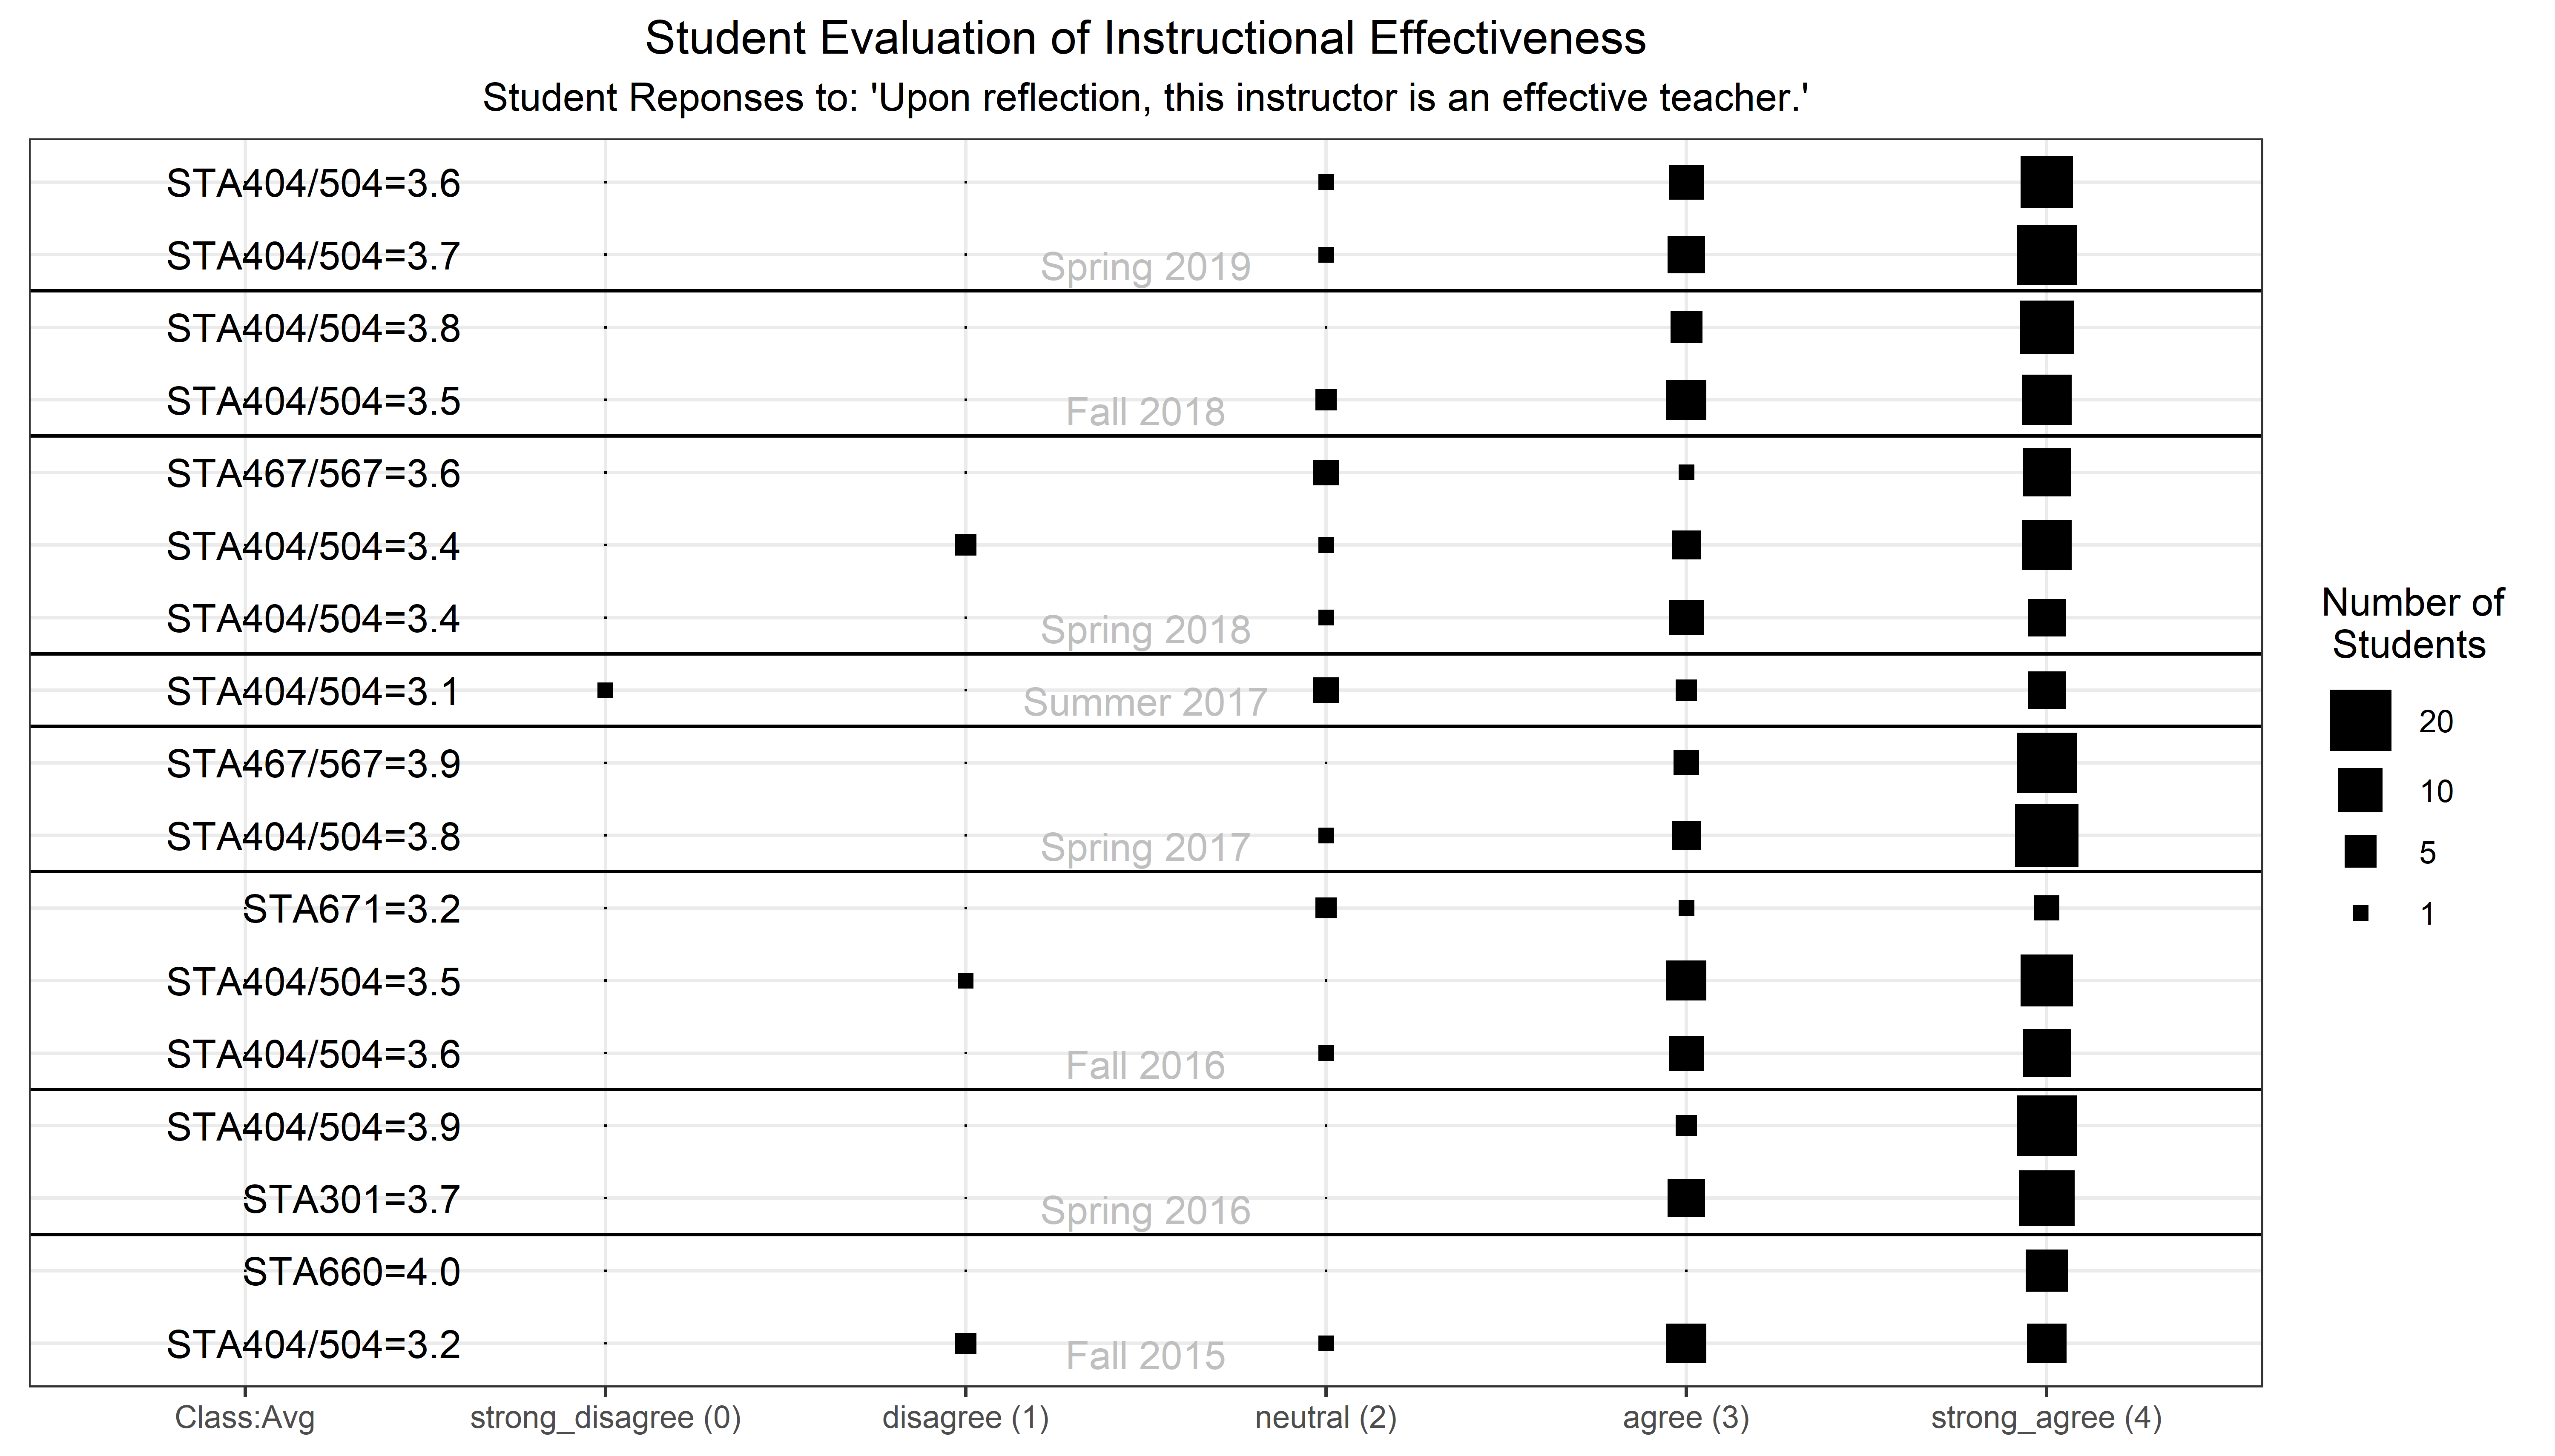
\includegraphics[width=1.2\textwidth]{CourseEvalPlotSpring2019.png}
\end{figure}
\end{center}

%----------------------------------------------------------------------------------------
  %  Publications Section
%----------------------------------------------------------------------------------------
  
  \section{PUBLICATION} 

\textbf{Maurer K.} Hudiburgh L., Werwinski L., Bailer A.J., (2019) [In-Press] {\it Content Audit for P-value Principles in Introductory Statistics} (The American Statistician)

\textbf{Maurer K.} Osthus D., Loy A., (2019) \href{https://rdcu.be/bgbJV}{\it A tale of four cities: exploring the soul of State College, Detroit, Milledgeville and Biloxi} (Computational Statistics) 

Garrett R., Nar A., Fisher T., \textbf{Maurer K.}, (2018) \href{https://www.theoj.org/joss-papers/joss.01096/10.21105.joss.01096.pdf}{\it ggvoronoi: Voronoi Diagrams and Heatmaps with ggplot2} (Journal of Open Source Software, 3(32), 1096) 

Alessio H., \textbf{Maurer K.}, (2018) \href{http://celt.muohio.edu/ject/fetch.php?id=734}{\it The Impact of Video Proctoring in Online Courses} (Journal on Excellence in College Teaching, 29(3&4)) 

Alessio H., Malay N., \textbf{Maurer K.}, Bailer J., Rubin B., (2018) \href{http://www.irrodl.org/index.php/irrodl/article/view/3698/4843}{\it Interaction of Proctoring and Student Major on Online Test Performance} (The International Review of Research in Open and Distributed Learning) 

Miljkovic T., Miljkovic D., \textbf{Maurer K.}, (2018) \href{https://link.springer.com/article/10.1007/s13385-018-0178-2}{\it Examining the Impact on Mortality Arising from Climate Change: Important Findings for the Insurance Industry} (European Actuarial Journal)

Alessio H., Malay N., \textbf{Maurer K.}, Bailer J., Rubin B. (2017), \href{https://olj.onlinelearningconsortium.org/index.php/olj/article/view/885}{{\it Examining the Effect of Proctoring on Online Test Scores}} (Online Learning Journal) 

\textbf{Maurer K.}, Lock D. (2016), \href{http://escholarship.org/uc/item/0wm523b0}{{\it Comparison of Learning Outcomes for Randomization-Based and Traditional Inference Curricula in a Designed Educational Experiment}} (Technology Innovations in Statistics Education, Volume 8)

%----------------------------------------------------------------------------------------
  %  Submitted MANUSCRIPTS Section
%----------------------------------------------------------------------------------------
  
  \section{SUBMITTED MANUSCRIPTS} 

\textbf{Maurer K.}, Bennette W., \textit{Facility Locations Utility for Uncovering Classifier Overconfidence} (ICML)

\textbf{Maurer K.}, Hudiburgh L., Werwinski L., \textit{Stake Your Claims: Comparing Probability Lab Activities using a Dice Game vs. Word Problems}  (Teaching Statistics)

\textbf{Maurer K.}, Hofmann H., {\it A \texttt{shiny} New Opportunity to Interact with Large Databases in Introductory Statistics} (TISE)

\textbf{Maurer K.}, {\it Iterative Quantile Nearest-Neighbors} (SCDA)



%----------------------------------------------------------------------------------------
  %  Manuscripts in Preparation Section
%---------------------------------------------------------------------------------------- 
  
\section{ONGOING RESEARCH PROJECTS}

Garrett R., Fisher T., \textbf{Maurer K.}, {\it Voronoi Diagram Applications}

Swart D., \textbf{Maurer K.}, Hudiburgh L., {\it Comparison of Instructor and Publisher Created Homework Sets for Introductory Statistics}  

Woodbury G., \textbf{Maurer K.}, Kim S., {\it Individual Visual Inference: Lady Tasting Tea Lineup Plots}

Grudsinski et al. {\it Beaver Dam Ecological Meta-Analysis}

\textbf{Maurer K.}, Bennette W., Wang Y., Underwood A., {\it Bin-Weighted Ensemble Classifiers}

\textbf{Maurer K.}, Vanderplas S., Hofmann H., {\it Developing and Evaluating Loss Functions for Binned Scatterplots Under Random and Standard Binning Algorithms} 
% \vspace{.05in}
%----------------------------------------------------------------------------------------
  %  Presentations Section
%---------------------------------------------------------------------------------------- 
  
  \section{PRESENTATION}

{\sl ``Iterative Quantile Nearest-Neigbhbors''} \hfill July 2018 \\
Joint Statistical Meetings, Vancouver BC

{\sl ``Fantasy Basketball For Statistical Learning''} \hfill May 2018 \\
Electronic Conference on Teaching Statistics, Online

{\sl ``Bin-Weighted Ensemble Classifiers''} \hfill July 2017 \\
Joint Statistical Meetings, Baltimore MD

{\sl ``Traditional vs. Simulation-Based:} \hfill August 2016 \\
{\sl  Curricula Comparison in a Small Scale Educational Experiment''}\\
Joint Statistical Meetings, Chicago IL

%----------------------------------------------------------------------------------------
  %	EXTRA-CURRICULAR ACTIVITIES SECTION
%----------------------------------------------------------------------------------------
  
  \section{UNIVERSITY SERVICE} 

{\it Member}, Dept. of Statistics TCPL Hiring Search Committee \hfill Spring 2019  \\
{\it Member}, CAS Committee on Big Ideas in Digital Media \hfill  Spring 2018 \\
{\it Member}, Dept. of Statistics Undergraduate Curriculum Committee \hfill  Spring 2018 \\
{\it Member}, Dept. of Statistics Grad Ed Committee \hfill  Fall 2016 - Present  \\
{\it Member}, Miami Datafest Committee \hfill  Fall 2015 - Present \\
{\it Member}, Dept. of Statistics Hiring Search Committee \hfill  Fall 2016  \\
{\it Panelist}, New Faculty Orientation Panel \hfill  Fall 2016 \\
{\it Volunteer}, Make It Miami Department Representative  \hfill  Spring 2016-Present  \\
{\it Volunteer}, Bridges Program Workshop Instructor  \hfill  Fall 2017-2018  \\
{\it Volunteer}, Careers Involving Quantitative Science (CIQS) Day  \hfill  Winter 2016-2018  

\section{PROFESSIONAL SERVICE} 
{\it Judge}, Undergraduate Research Project Competition \hfill  Summer 2016 \\
{\it Peer Reviewer}, Journal for Statistical Education \hfill  Spring 2016 - Present  \\

\section{COMMUNITY SERVICE} 
{\it Instructor}, Client Data Visualization Projects \hfill  Fall 2015 - Spring 2017 
\begin{itemize} \itemsep -2pt
\item Miami EHWB - \href{http://dataviz.miamioh.edu/DataVizClassFall2015/MiamiEmployeeHealthApps/EmployeeGymUsage/}{Gym and Benefit Usage App}
\item Cincinnati Shakespeare Co. - \href{http://dataviz.miamioh.edu/Shakespeare/}{Ticket Sales App (Redesign)}
\item Butler County Health - \href{http://dataviz.miamioh.edu/BCH/Butler_County_Infant_Mortality/}{Interactive Infant Mortality Report App}
\item St. Louis County EMS - \href{http://dataviz.miamioh.edu/Minnesota_EMS/}{Emergency Response Times App}
\item Scripps Gerontology Center - \href{http://dataviz.miamioh.edu/DataVizClassFall2015/OhioNursingSurveyApps/EmployeeSafety/}{Nursing Facility Survey App}
\end{itemize}

%----------------------------------------------------------------------------------------
  %	EXTRA-CURRICULAR ACTIVITIES SECTION
%----------------------------------------------------------------------------------------
  
  \section{OTHER EXPERIENCE} 

{\it Member}, Miami University NFRC \hfill  Fall 2016 \\
{\it Member}, Miami University NFTEP \hfill  Spring 2016  \\

%----------------------------------------------------------------------------------------
  
  \end{resume}
\end{document}
